\documentclass[a4paper]{article}
\usepackage{amsmath}
\usepackage{graphicx}
\usepackage{longtable}
\usepackage{makecell}
\usepackage[most]{tcolorbox}
\usepackage{listings}
\usepackage{csquotes}

\title{SDCND Advanced Lane Finding}
\date{2019-03-11}
\author{Matthias Schinacher matthias.schinacher@googlemail.com}

\begin{document}

\maketitle
\tableofcontents
\newpage

\section{Intro}
The project is a homework assignment for Udacity's \textbf{Self Driving Car Nano Degree}.
The project is the second one called \textit{Advanced Lane Finding}.

\subsection{Implementation}
I choose to implement the necessary code as a series of python scripts invoked from
the command line, rather than implementing a notebook. I did use however the
example \texttt{example.ipynb} as a starting point for the calibration.
\\
I also used my versions of the solutions to the various quizzes in the course
as a code base for my scripts.
\\
The scripts implement each a specific part of the required task for the
project. Those scripts that produce results used in later stages, use the
standard python \textit{pickle} module to save data as python objects.
\\
The scripts have positional command-line parameters.

\section{Calibration}
I calibrated the \enquote{camera} with the script texttt{calibrate.py}.
It uses the \texttt{cv2} method \texttt{calibrateCamera(...)} to do the actual
calibration and \texttt{findChessboardCorners(...)} to find the image points
required within the given chessboard calibration pictures.
\\
The calibration matrix etc. computed is written to a pickle file and the
scripts allows to save and/or show modified calibration images, onto which
the actual chess board corners (\texttt{findChessboardCorners(...)})
are drawn.

\paragraph{Script parameters}
:\\
\small
\begin{tabular}{ |c|l|l|c| }
  \hline
Position & Name & Description & Default \\
  \hline
1 & \texttt{show-flag} & show the modified calibration images? & \texttt{False} \\
2 & \texttt{save-flag} & save the modified calibration images? & \texttt{True} \\
3 & \texttt{pickle-file-name} & picke file name & \texttt{calibration.pickle} \\
\hline
\end{tabular}
\normalsize
\textit{(the \enquote{save-flag} is only for the pictures, the pickle file will always be written)}

\paragraph{Graphs}
\textit{(some examples of the chessboard corners found in the calibration images)}
:\\
\begin{tabular}{ |c|c| }
  \hline
  Calibration picture & ... with corners identified \\
  \hline
  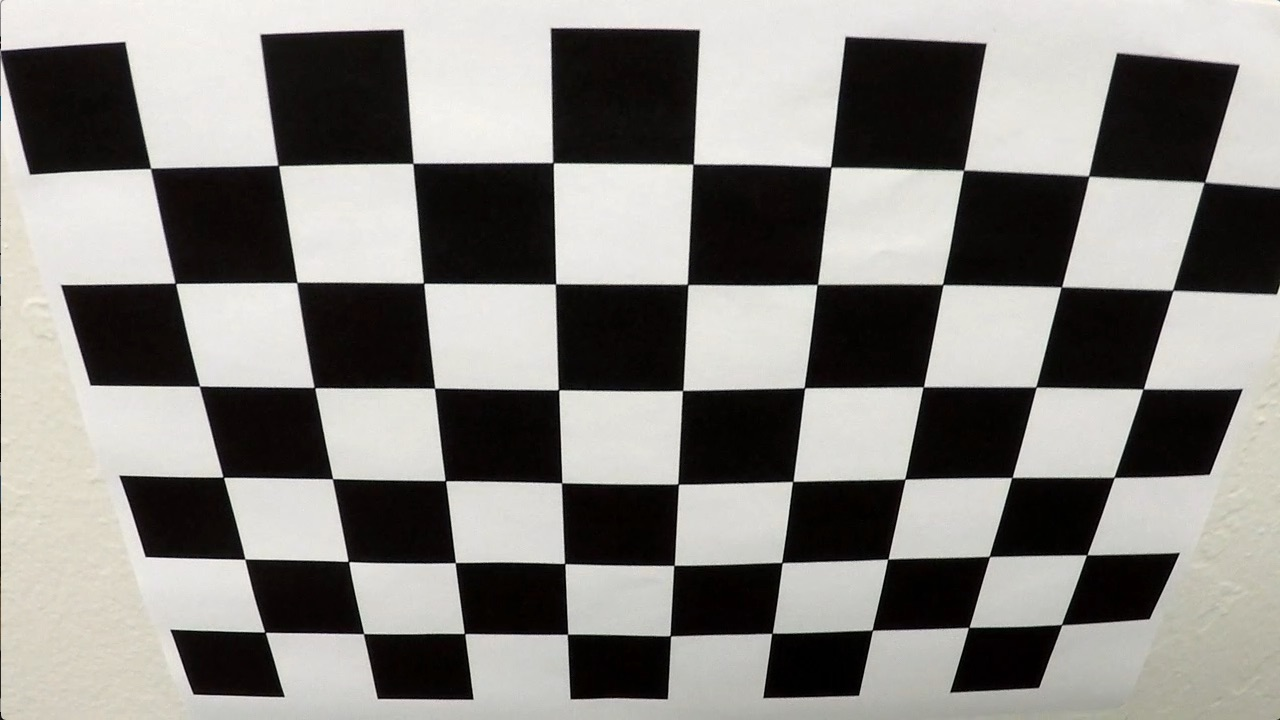
\includegraphics[scale=0.15]{calibration2.jpg} & \includegraphics[scale=0.15]{modcalibration2.jpg} \\
  \hline
  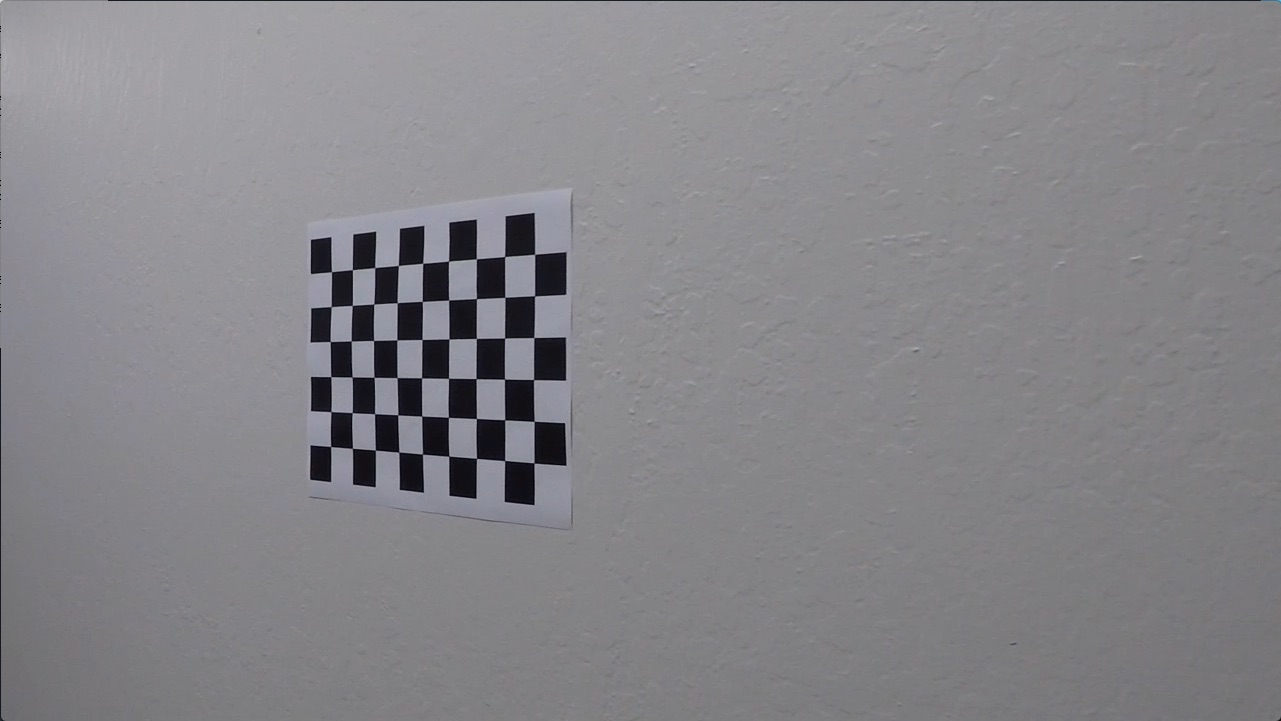
\includegraphics[scale=0.15]{calibration7.jpg} & \includegraphics[scale=0.15]{modcalibration7.jpg} \\
  \hline
  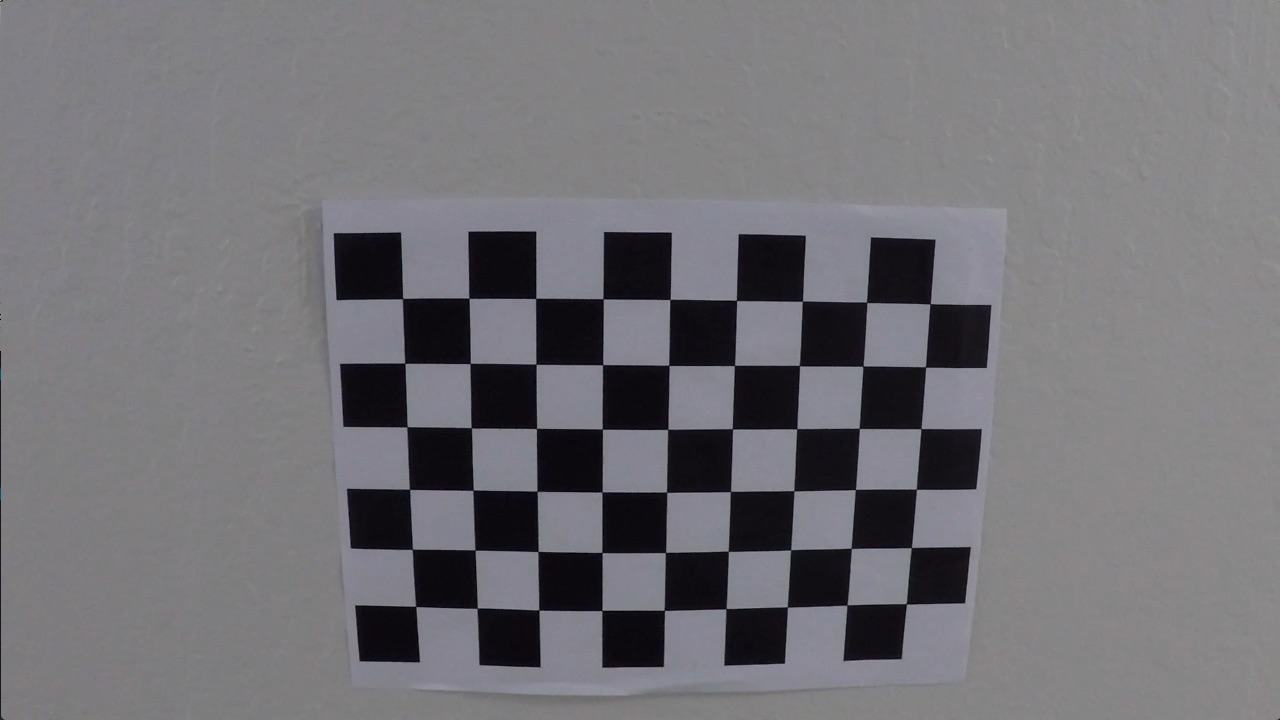
\includegraphics[scale=0.15]{calibration17.jpg} & \includegraphics[scale=0.15]{modcalibration17.jpg} \\
  \hline
\end{tabular}
\\
\textbf{Note:} creation of actual undistorted images is done by the additional script
\texttt{undistort.py}, which reads the calibration parameters from the pickle file
(see source for required params).
\\

\textit{(same examples with undistorted images)}
:\\
\begin{tabular}{ |c|c| }
  \hline
  Calibration picture & ... with corners identified \\
  \hline
  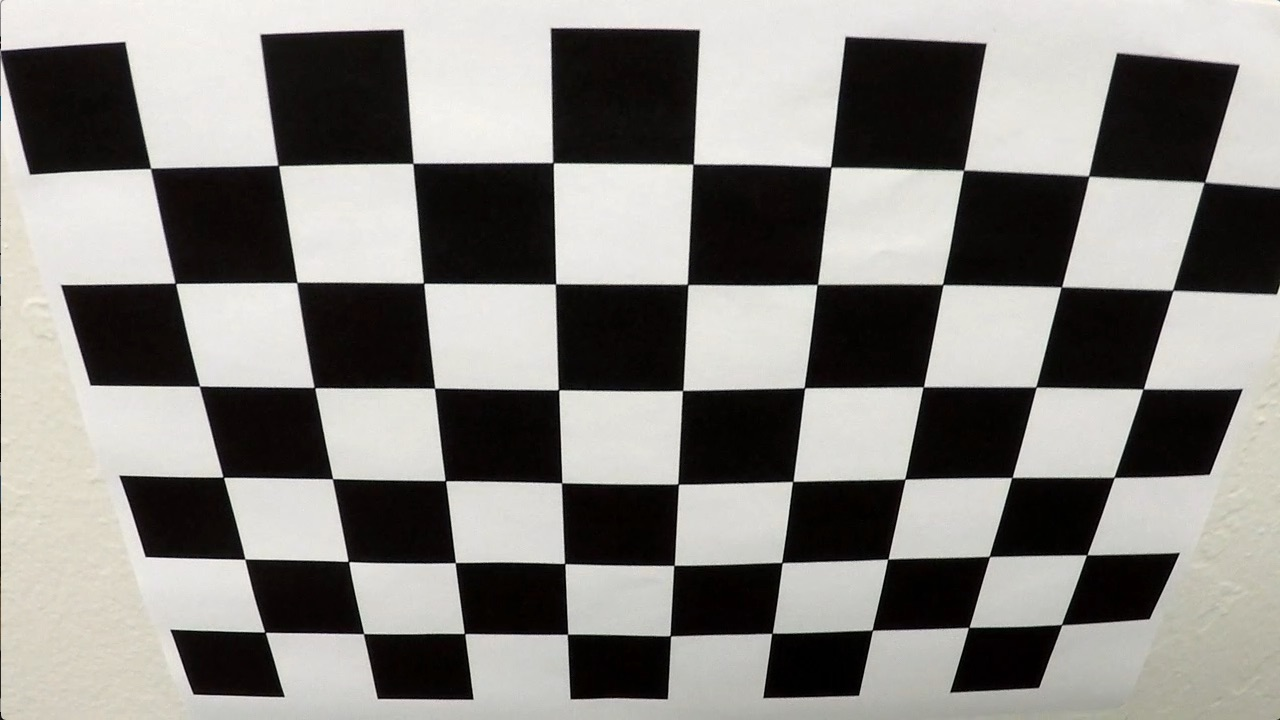
\includegraphics[scale=0.15]{calibration2.jpg} & \includegraphics[scale=0.15]{udcalibration2.jpg} \\
  \hline
  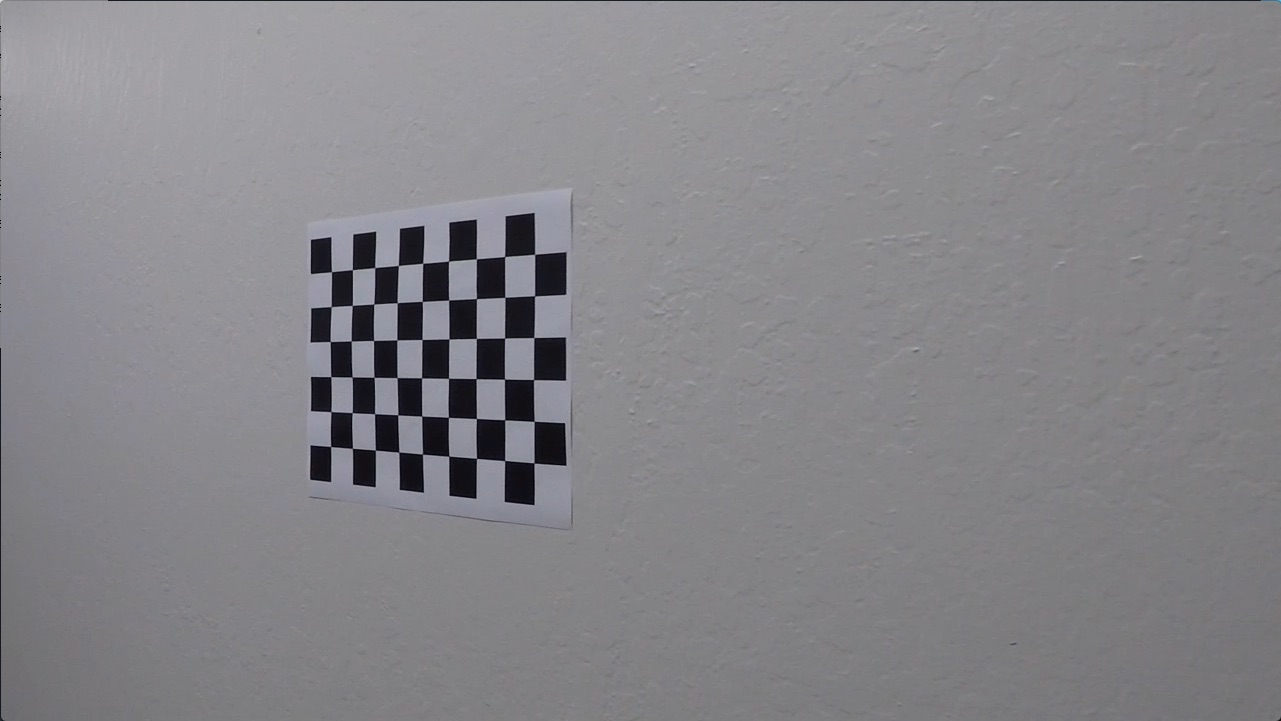
\includegraphics[scale=0.15]{calibration7.jpg} & \includegraphics[scale=0.15]{udcalibration7.jpg} \\
  \hline
  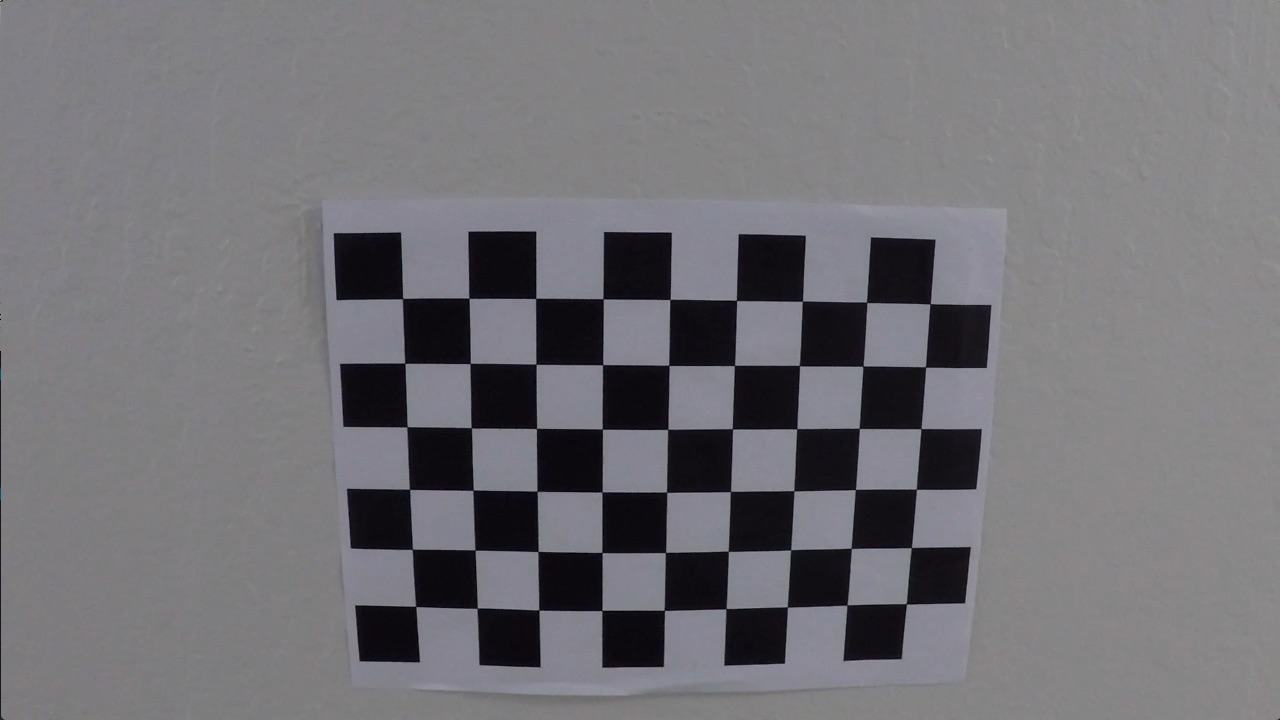
\includegraphics[scale=0.15]{calibration17.jpg} & \includegraphics[scale=0.15]{udcalibration17.jpg} \\
  \hline
\end{tabular}

\section{Perspective transform}
To find a good perspective transform I implemented the script \texttt{transform.py};
It takes as positional input parameters the x and y coordinates for a source quadrilateral
and a destination rectangle defining the desired transform.
\\
Additional parameters control whether to show the test images and how they transform
on the screen and potentially save transformed images and the transformation
parameters (in a pickle file).
\\
This allowed me to experiment with a number of different transformations quite rapidly.
The \enquote{best} transform I came up with \textit{(dubbed \enquote{MA})}, was derived
from the first picture \textit{with straight lines}.
\\
To get the coordinates for the source quadrilateral I would usually open one of
the \textit{straight lines}- pictures with gimp to identify 4 corners that were
not a rectangle but would obviously be close to one in the real. I would then
experiment with a couple of target rectangle coordinates.

\paragraph{Script parameters}
:\\
\small
\begin{tabular}{ |c|l|l|c| }
  \hline
Position & Name & Description & Default \\
  \hline
1 & \texttt{transformation-name} &  & (\textit{mandatory}) \\
2 & \texttt{cooordinate-string} &  & (\textit{mandatory}) \\
3 & \texttt{show-flag} & show images? & \texttt{False} \\
4 & \texttt{save-flag} & save images? & \texttt{False} \\
\hline
\end{tabular}
\normalsize
\\
The coordinates must be given as 16 integers within one string; that requires
the string to be in quotes on the command line, like:\\
\tiny
\texttt{python transform.py MA '425 570 1276 570 806 458 586 458  325 600 1076 600 1076 100 325 100' 1 1}
\normalsize

\paragraph{Graphs}
\textit{(some examples perspective transform; source to transformed picture
with the areas from the transform definition marked.)}
:\\
\begin{tabular}{ |c|c| }
  \hline
  source & transformed \\
  \hline
  \multicolumn{2}{|c|}{\texttt{straight\_lines1.jpg}} \\
  \includegraphics[scale=0.15]{source01.jpg} & \includegraphics[scale=0.15]{transformed01.jpg} \\
  \hline
  \multicolumn{2}{|c|}{\texttt{straight\_lines2.jpg}} \\
  \includegraphics[scale=0.15]{source02.jpg} & \includegraphics[scale=0.15]{transformed02.jpg} \\
  \hline
  \multicolumn{2}{|c|}{\texttt{test3.jpg}} \\
  \includegraphics[scale=0.15]{source03.jpg} & \includegraphics[scale=0.15]{transformed03.jpg} \\
  \hline
\end{tabular}

\section{Pipeline}
The pipeline to actually process the whole lane finding is mainly implemented
in the python sources \texttt{sliding\_window.py} (helper functions/ methods
for the sliding window approach) and \texttt{single\_image\_pipeline.py}.
\\
The latter contains most of the functionality including the reading/ writing of
a parameter file (which uses pythons \texttt{configparser}).
\\
If called directly it allows for the processing of the test images or a single
image (depending on positional parameter) by the pipeline, while the various
steps resulting images are shown and/or saved to image files.
This allowed for experimentation with different parameter sets through the use
of parameter files (which also \enquote{recorded} the parameters used).
\\
The script to create the videos (\texttt{clip\_pipeline.py}) is mainly a wrapper
around the pipeline for single images, only with the function/ method- arguments
set in a way, so that no direct image showing or saving is attempted (as the
images are not to be saved individually, but as part of a video stream).

\subsection{Pipeline overview}
The images undergo following steps:
\begin{itemize}
\item Distortion correction (using the values from the calibration)
\item Conversion to HLS and using only the S channel after that
\item Thresholding the S- channel
\item Sobel processing with a combination of magnitude and directional thresholding
\item Canny
\item Masking with a polygon
\item Hough lines
\item Perspective transform
\item Sliding window processing with second order polynomial fit
\item Filling of the lane (green) in transformed coordinates given the fitting functions
\item Retransformation of the picture and combining with original image
\end{itemize}

\subsection{Example graphics}
The pipeline visualized on test- image \texttt{test6.jpg}
:\\
\small
\begin{tabular}{ |c|c|c }
  \hline
  original image & $\rightarrow$ undistorted image & $\rightarrow$ S channel (of HLS) \\
  \includegraphics[scale=0.1]{test6-01.jpg} & \includegraphics[scale=0.1]{test6-U.jpg} & \includegraphics[scale=0.1]{test6-S.jpg} \\
  $\rightarrow$ S- channel thresholded & $\rightarrow$ after sobel & $\rightarrow$ after canny \\
  \includegraphics[scale=0.1]{test6-S2.jpg} & \includegraphics[scale=0.1]{test6-SOB.jpg} & \includegraphics[scale=0.1]{test6-C.jpg} \\
  $\rightarrow$ masking & $\rightarrow$ hough lines & $\rightarrow$ after perspective trans. \\
  \includegraphics[scale=0.1]{test6-M.jpg} & \includegraphics[scale=0.1]{test6-H.jpg} & \includegraphics[scale=0.1]{test6-W.jpg} \\
  $\rightarrow$ sliding windows & $\rightarrow$ final combined image & \\
  \includegraphics[scale=0.1]{test6-SW.jpg} & \includegraphics[scale=0.1]{test6-final.jpg} &  \\
  \hline
\end{tabular}

The parameters used are from \texttt{params\_05.ini}.

\subsection{Video}
Up until now I could only half successfully convert the first 45 seconds of the
\texttt{project\_video.mp4}, see respective output folder.

\section{Discussion}
I was a bit frustrated, because I could not find a set of parameters (within
my limited time), that would yield a pipeline robust enough for my taste.
\\
While the implementation seems to work well enough on single images (see the
graphics for \texttt{test6.jpg} above), the application to video yields a
lane marking way too shaky. I tried to remedy this by remembering the starting
positions for the sliding window processing from frame to frame (say: image
to next image) and even implemented a scheme as to reuse the last polynomial
fits with a certain fraction (30 percent) to smooth the computation;
did not really help much.
\\
The main problem seems to me, that the intermittent lane markings are not
identified/ spotted well enough.

\subsection{Possible improvements}
I would make an educated guess, that extensive experimentation with different
parameters for the various steps could be helpful. I think especially the
\enquote{right} combination of parameters for the \textit{canny- step}, the
masking polygon and the hough-line processing might be promising (
\textit{I would actually need to implement the parameters for the masking
polygon to be read from config - as the mask is hard coded as of now}).
\\
To improve the lane detection within the context of the video, I would maybe
experiment with something like \enquote{carrying over} a fraction of the
sliding window pixels from the last frame randomly, but only those within the
boxes; this might improve the stability of the polynomial fit (because
more data points are available).

\end{document}
